
% Default to the notebook output style




% Inherit from the specified cell style.





\documentclass[11pt]{article}
    \pagenumbering{gobble}



    \usepackage[T1]{fontenc}
    % Nicer default font (+ math font) than Computer Modern for most use cases
    \usepackage{mathpazo}

    % Basic figure setup, for now with no caption control since it's done
    % automatically by Pandoc (which extracts ![](path) syntax from Markdown).
    \usepackage{graphicx}
    % We will generate all images so they have a width \maxwidth. This means
    % that they will get their normal width if they fit onto the page, but
    % are scaled down if they would overflow the margins.
    \makeatletter
    \def\maxwidth{\ifdim\Gin@nat@width>\linewidth\linewidth
    \else\Gin@nat@width\fi}
    \makeatother
    \let\Oldincludegraphics\includegraphics
    % Set max figure width to be 80% of text width, for now hardcoded.
    \renewcommand{\includegraphics}[1]{\Oldincludegraphics[width=.8\maxwidth]{#1}}
    % Ensure that by default, figures have no caption (until we provide a
    % proper Figure object with a Caption API and a way to capture that
    % in the conversion process - todo).
    \usepackage{caption}
    \DeclareCaptionLabelFormat{nolabel}{}
    \captionsetup{labelformat=nolabel}

    \usepackage{adjustbox} % Used to constrain images to a maximum size
    \usepackage{xcolor} % Allow colors to be defined
    \usepackage{enumerate} % Needed for markdown enumerations to work
    \usepackage{geometry} % Used to adjust the document margins
    \usepackage{amsmath} % Equations
    \usepackage{amssymb} % Equations
    \usepackage{textcomp} % defines textquotesingle
    % Hack from http://tex.stackexchange.com/a/47451/13684:
    \AtBeginDocument{%
        \def\PYZsq{\textquotesingle}% Upright quotes in Pygmentized code
    }
    \usepackage{upquote} % Upright quotes for verbatim code
    \usepackage{eurosym} % defines \euro
    \usepackage[mathletters]{ucs} % Extended unicode (utf-8) support
    \usepackage[utf8x]{inputenc} % Allow utf-8 characters in the tex document
    \usepackage{fancyvrb} % verbatim replacement that allows latex
    \usepackage{grffile} % extends the file name processing of package graphics
                         % to support a larger range
    % The hyperref package gives us a pdf with properly built
    % internal navigation ('pdf bookmarks' for the table of contents,
    % internal cross-reference links, web links for URLs, etc.)
    \usepackage{hyperref}
    \usepackage{longtable} % longtable support required by pandoc >1.10
    \usepackage{booktabs}  % table support for pandoc > 1.12.2
    \usepackage[inline]{enumitem} % IRkernel/repr support (it uses the enumerate* environment)
    \usepackage[normalem]{ulem} % ulem is needed to support strikethroughs (\sout)
                                % normalem makes italics be italics, not underlines




    % Colors for the hyperref package
    \definecolor{urlcolor}{rgb}{0,.145,.698}
    \definecolor{linkcolor}{rgb}{.71,0.21,0.01}
    \definecolor{citecolor}{rgb}{.12,.54,.11}

    % ANSI colors
    \definecolor{ansi-black}{HTML}{3E424D}
    \definecolor{ansi-black-intense}{HTML}{282C36}
    \definecolor{ansi-red}{HTML}{E75C58}
    \definecolor{ansi-red-intense}{HTML}{B22B31}
    \definecolor{ansi-green}{HTML}{00A250}
    \definecolor{ansi-green-intense}{HTML}{007427}
    \definecolor{ansi-yellow}{HTML}{DDB62B}
    \definecolor{ansi-yellow-intense}{HTML}{B27D12}
    \definecolor{ansi-blue}{HTML}{208FFB}
    \definecolor{ansi-blue-intense}{HTML}{0065CA}
    \definecolor{ansi-magenta}{HTML}{D160C4}
    \definecolor{ansi-magenta-intense}{HTML}{A03196}
    \definecolor{ansi-cyan}{HTML}{60C6C8}
    \definecolor{ansi-cyan-intense}{HTML}{258F8F}
    \definecolor{ansi-white}{HTML}{C5C1B4}
    \definecolor{ansi-white-intense}{HTML}{A1A6B2}

    % commands and environments needed by pandoc snippets
    % extracted from the output of `pandoc -s`
    \providecommand{\tightlist}{%
      \setlength{\itemsep}{0pt}\setlength{\parskip}{0pt}}
    \DefineVerbatimEnvironment{Highlighting}{Verbatim}{commandchars=\\\{\}}
    % Add ',fontsize=\small' for more characters per line
    \newenvironment{Shaded}{}{}
    \newcommand{\KeywordTok}[1]{\textcolor[rgb]{0.00,0.44,0.13}{\textbf{{#1}}}}
    \newcommand{\DataTypeTok}[1]{\textcolor[rgb]{0.56,0.13,0.00}{{#1}}}
    \newcommand{\DecValTok}[1]{\textcolor[rgb]{0.25,0.63,0.44}{{#1}}}
    \newcommand{\BaseNTok}[1]{\textcolor[rgb]{0.25,0.63,0.44}{{#1}}}
    \newcommand{\FloatTok}[1]{\textcolor[rgb]{0.25,0.63,0.44}{{#1}}}
    \newcommand{\CharTok}[1]{\textcolor[rgb]{0.25,0.44,0.63}{{#1}}}
    \newcommand{\StringTok}[1]{\textcolor[rgb]{0.25,0.44,0.63}{{#1}}}
    \newcommand{\CommentTok}[1]{\textcolor[rgb]{0.38,0.63,0.69}{\textit{{#1}}}}
    \newcommand{\OtherTok}[1]{\textcolor[rgb]{0.00,0.44,0.13}{{#1}}}
    \newcommand{\AlertTok}[1]{\textcolor[rgb]{1.00,0.00,0.00}{\textbf{{#1}}}}
    \newcommand{\FunctionTok}[1]{\textcolor[rgb]{0.02,0.16,0.49}{{#1}}}
    \newcommand{\RegionMarkerTok}[1]{{#1}}
    \newcommand{\ErrorTok}[1]{\textcolor[rgb]{1.00,0.00,0.00}{\textbf{{#1}}}}
    \newcommand{\NormalTok}[1]{{#1}}

    % Additional commands for more recent versions of Pandoc
    \newcommand{\ConstantTok}[1]{\textcolor[rgb]{0.53,0.00,0.00}{{#1}}}
    \newcommand{\SpecialCharTok}[1]{\textcolor[rgb]{0.25,0.44,0.63}{{#1}}}
    \newcommand{\VerbatimStringTok}[1]{\textcolor[rgb]{0.25,0.44,0.63}{{#1}}}
    \newcommand{\SpecialStringTok}[1]{\textcolor[rgb]{0.73,0.40,0.53}{{#1}}}
    \newcommand{\ImportTok}[1]{{#1}}
    \newcommand{\DocumentationTok}[1]{\textcolor[rgb]{0.73,0.13,0.13}{\textit{{#1}}}}
    \newcommand{\AnnotationTok}[1]{\textcolor[rgb]{0.38,0.63,0.69}{\textbf{\textit{{#1}}}}}
    \newcommand{\CommentVarTok}[1]{\textcolor[rgb]{0.38,0.63,0.69}{\textbf{\textit{{#1}}}}}
    \newcommand{\VariableTok}[1]{\textcolor[rgb]{0.10,0.09,0.49}{{#1}}}
    \newcommand{\ControlFlowTok}[1]{\textcolor[rgb]{0.00,0.44,0.13}{\textbf{{#1}}}}
    \newcommand{\OperatorTok}[1]{\textcolor[rgb]{0.40,0.40,0.40}{{#1}}}
    \newcommand{\BuiltInTok}[1]{{#1}}
    \newcommand{\ExtensionTok}[1]{{#1}}
    \newcommand{\PreprocessorTok}[1]{\textcolor[rgb]{0.74,0.48,0.00}{{#1}}}
    \newcommand{\AttributeTok}[1]{\textcolor[rgb]{0.49,0.56,0.16}{{#1}}}
    \newcommand{\InformationTok}[1]{\textcolor[rgb]{0.38,0.63,0.69}{\textbf{\textit{{#1}}}}}
    \newcommand{\WarningTok}[1]{\textcolor[rgb]{0.38,0.63,0.69}{\textbf{\textit{{#1}}}}}


    % Define a nice break command that doesn't care if a line doesn't already
    % exist.
    \def\br{\hspace*{\fill} \\* }
    % Math Jax compatability definitions
    \def\gt{>}
    \def\lt{<}
    % Document parameters
    \title{MoS2 Background}
    \date{}




    % Pygments definitions

\makeatletter
\def\PY@reset{\let\PY@it=\relax \let\PY@bf=\relax%
    \let\PY@ul=\relax \let\PY@tc=\relax%
    \let\PY@bc=\relax \let\PY@ff=\relax}
\def\PY@tok#1{\csname PY@tok@#1\endcsname}
\def\PY@toks#1+{\ifx\relax#1\empty\else%
    \PY@tok{#1}\expandafter\PY@toks\fi}
\def\PY@do#1{\PY@bc{\PY@tc{\PY@ul{%
    \PY@it{\PY@bf{\PY@ff{#1}}}}}}}
\def\PY#1#2{\PY@reset\PY@toks#1+\relax+\PY@do{#2}}

\expandafter\def\csname PY@tok@fm\endcsname{\def\PY@tc##1{\textcolor[rgb]{0.00,0.00,1.00}{##1}}}
\expandafter\def\csname PY@tok@c\endcsname{\let\PY@it=\textit\def\PY@tc##1{\textcolor[rgb]{0.25,0.50,0.50}{##1}}}
\expandafter\def\csname PY@tok@ge\endcsname{\let\PY@it=\textit}
\expandafter\def\csname PY@tok@nc\endcsname{\let\PY@bf=\textbf\def\PY@tc##1{\textcolor[rgb]{0.00,0.00,1.00}{##1}}}
\expandafter\def\csname PY@tok@si\endcsname{\let\PY@bf=\textbf\def\PY@tc##1{\textcolor[rgb]{0.73,0.40,0.53}{##1}}}
\expandafter\def\csname PY@tok@cs\endcsname{\let\PY@it=\textit\def\PY@tc##1{\textcolor[rgb]{0.25,0.50,0.50}{##1}}}
\expandafter\def\csname PY@tok@kr\endcsname{\let\PY@bf=\textbf\def\PY@tc##1{\textcolor[rgb]{0.00,0.50,0.00}{##1}}}
\expandafter\def\csname PY@tok@sb\endcsname{\def\PY@tc##1{\textcolor[rgb]{0.73,0.13,0.13}{##1}}}
\expandafter\def\csname PY@tok@s\endcsname{\def\PY@tc##1{\textcolor[rgb]{0.73,0.13,0.13}{##1}}}
\expandafter\def\csname PY@tok@gp\endcsname{\let\PY@bf=\textbf\def\PY@tc##1{\textcolor[rgb]{0.00,0.00,0.50}{##1}}}
\expandafter\def\csname PY@tok@vg\endcsname{\def\PY@tc##1{\textcolor[rgb]{0.10,0.09,0.49}{##1}}}
\expandafter\def\csname PY@tok@nd\endcsname{\def\PY@tc##1{\textcolor[rgb]{0.67,0.13,1.00}{##1}}}
\expandafter\def\csname PY@tok@mo\endcsname{\def\PY@tc##1{\textcolor[rgb]{0.40,0.40,0.40}{##1}}}
\expandafter\def\csname PY@tok@gu\endcsname{\let\PY@bf=\textbf\def\PY@tc##1{\textcolor[rgb]{0.50,0.00,0.50}{##1}}}
\expandafter\def\csname PY@tok@s2\endcsname{\def\PY@tc##1{\textcolor[rgb]{0.73,0.13,0.13}{##1}}}
\expandafter\def\csname PY@tok@mh\endcsname{\def\PY@tc##1{\textcolor[rgb]{0.40,0.40,0.40}{##1}}}
\expandafter\def\csname PY@tok@nf\endcsname{\def\PY@tc##1{\textcolor[rgb]{0.00,0.00,1.00}{##1}}}
\expandafter\def\csname PY@tok@vc\endcsname{\def\PY@tc##1{\textcolor[rgb]{0.10,0.09,0.49}{##1}}}
\expandafter\def\csname PY@tok@bp\endcsname{\def\PY@tc##1{\textcolor[rgb]{0.00,0.50,0.00}{##1}}}
\expandafter\def\csname PY@tok@mb\endcsname{\def\PY@tc##1{\textcolor[rgb]{0.40,0.40,0.40}{##1}}}
\expandafter\def\csname PY@tok@sx\endcsname{\def\PY@tc##1{\textcolor[rgb]{0.00,0.50,0.00}{##1}}}
\expandafter\def\csname PY@tok@nv\endcsname{\def\PY@tc##1{\textcolor[rgb]{0.10,0.09,0.49}{##1}}}
\expandafter\def\csname PY@tok@sh\endcsname{\def\PY@tc##1{\textcolor[rgb]{0.73,0.13,0.13}{##1}}}
\expandafter\def\csname PY@tok@gd\endcsname{\def\PY@tc##1{\textcolor[rgb]{0.63,0.00,0.00}{##1}}}
\expandafter\def\csname PY@tok@o\endcsname{\def\PY@tc##1{\textcolor[rgb]{0.40,0.40,0.40}{##1}}}
\expandafter\def\csname PY@tok@no\endcsname{\def\PY@tc##1{\textcolor[rgb]{0.53,0.00,0.00}{##1}}}
\expandafter\def\csname PY@tok@c1\endcsname{\let\PY@it=\textit\def\PY@tc##1{\textcolor[rgb]{0.25,0.50,0.50}{##1}}}
\expandafter\def\csname PY@tok@dl\endcsname{\def\PY@tc##1{\textcolor[rgb]{0.73,0.13,0.13}{##1}}}
\expandafter\def\csname PY@tok@na\endcsname{\def\PY@tc##1{\textcolor[rgb]{0.49,0.56,0.16}{##1}}}
\expandafter\def\csname PY@tok@vm\endcsname{\def\PY@tc##1{\textcolor[rgb]{0.10,0.09,0.49}{##1}}}
\expandafter\def\csname PY@tok@go\endcsname{\def\PY@tc##1{\textcolor[rgb]{0.53,0.53,0.53}{##1}}}
\expandafter\def\csname PY@tok@cpf\endcsname{\let\PY@it=\textit\def\PY@tc##1{\textcolor[rgb]{0.25,0.50,0.50}{##1}}}
\expandafter\def\csname PY@tok@m\endcsname{\def\PY@tc##1{\textcolor[rgb]{0.40,0.40,0.40}{##1}}}
\expandafter\def\csname PY@tok@ch\endcsname{\let\PY@it=\textit\def\PY@tc##1{\textcolor[rgb]{0.25,0.50,0.50}{##1}}}
\expandafter\def\csname PY@tok@sd\endcsname{\let\PY@it=\textit\def\PY@tc##1{\textcolor[rgb]{0.73,0.13,0.13}{##1}}}
\expandafter\def\csname PY@tok@kd\endcsname{\let\PY@bf=\textbf\def\PY@tc##1{\textcolor[rgb]{0.00,0.50,0.00}{##1}}}
\expandafter\def\csname PY@tok@mi\endcsname{\def\PY@tc##1{\textcolor[rgb]{0.40,0.40,0.40}{##1}}}
\expandafter\def\csname PY@tok@nl\endcsname{\def\PY@tc##1{\textcolor[rgb]{0.63,0.63,0.00}{##1}}}
\expandafter\def\csname PY@tok@nb\endcsname{\def\PY@tc##1{\textcolor[rgb]{0.00,0.50,0.00}{##1}}}
\expandafter\def\csname PY@tok@il\endcsname{\def\PY@tc##1{\textcolor[rgb]{0.40,0.40,0.40}{##1}}}
\expandafter\def\csname PY@tok@mf\endcsname{\def\PY@tc##1{\textcolor[rgb]{0.40,0.40,0.40}{##1}}}
\expandafter\def\csname PY@tok@s1\endcsname{\def\PY@tc##1{\textcolor[rgb]{0.73,0.13,0.13}{##1}}}
\expandafter\def\csname PY@tok@kn\endcsname{\let\PY@bf=\textbf\def\PY@tc##1{\textcolor[rgb]{0.00,0.50,0.00}{##1}}}
\expandafter\def\csname PY@tok@ss\endcsname{\def\PY@tc##1{\textcolor[rgb]{0.10,0.09,0.49}{##1}}}
\expandafter\def\csname PY@tok@sc\endcsname{\def\PY@tc##1{\textcolor[rgb]{0.73,0.13,0.13}{##1}}}
\expandafter\def\csname PY@tok@err\endcsname{\def\PY@bc##1{\setlength{\fboxsep}{0pt}\fcolorbox[rgb]{1.00,0.00,0.00}{1,1,1}{\strut ##1}}}
\expandafter\def\csname PY@tok@se\endcsname{\let\PY@bf=\textbf\def\PY@tc##1{\textcolor[rgb]{0.73,0.40,0.13}{##1}}}
\expandafter\def\csname PY@tok@gh\endcsname{\let\PY@bf=\textbf\def\PY@tc##1{\textcolor[rgb]{0.00,0.00,0.50}{##1}}}
\expandafter\def\csname PY@tok@gs\endcsname{\let\PY@bf=\textbf}
\expandafter\def\csname PY@tok@kp\endcsname{\def\PY@tc##1{\textcolor[rgb]{0.00,0.50,0.00}{##1}}}
\expandafter\def\csname PY@tok@nt\endcsname{\let\PY@bf=\textbf\def\PY@tc##1{\textcolor[rgb]{0.00,0.50,0.00}{##1}}}
\expandafter\def\csname PY@tok@kc\endcsname{\let\PY@bf=\textbf\def\PY@tc##1{\textcolor[rgb]{0.00,0.50,0.00}{##1}}}
\expandafter\def\csname PY@tok@w\endcsname{\def\PY@tc##1{\textcolor[rgb]{0.73,0.73,0.73}{##1}}}
\expandafter\def\csname PY@tok@ni\endcsname{\let\PY@bf=\textbf\def\PY@tc##1{\textcolor[rgb]{0.60,0.60,0.60}{##1}}}
\expandafter\def\csname PY@tok@cp\endcsname{\def\PY@tc##1{\textcolor[rgb]{0.74,0.48,0.00}{##1}}}
\expandafter\def\csname PY@tok@vi\endcsname{\def\PY@tc##1{\textcolor[rgb]{0.10,0.09,0.49}{##1}}}
\expandafter\def\csname PY@tok@kt\endcsname{\def\PY@tc##1{\textcolor[rgb]{0.69,0.00,0.25}{##1}}}
\expandafter\def\csname PY@tok@sa\endcsname{\def\PY@tc##1{\textcolor[rgb]{0.73,0.13,0.13}{##1}}}
\expandafter\def\csname PY@tok@gr\endcsname{\def\PY@tc##1{\textcolor[rgb]{1.00,0.00,0.00}{##1}}}
\expandafter\def\csname PY@tok@cm\endcsname{\let\PY@it=\textit\def\PY@tc##1{\textcolor[rgb]{0.25,0.50,0.50}{##1}}}
\expandafter\def\csname PY@tok@gt\endcsname{\def\PY@tc##1{\textcolor[rgb]{0.00,0.27,0.87}{##1}}}
\expandafter\def\csname PY@tok@k\endcsname{\let\PY@bf=\textbf\def\PY@tc##1{\textcolor[rgb]{0.00,0.50,0.00}{##1}}}
\expandafter\def\csname PY@tok@sr\endcsname{\def\PY@tc##1{\textcolor[rgb]{0.73,0.40,0.53}{##1}}}
\expandafter\def\csname PY@tok@gi\endcsname{\def\PY@tc##1{\textcolor[rgb]{0.00,0.63,0.00}{##1}}}
\expandafter\def\csname PY@tok@nn\endcsname{\let\PY@bf=\textbf\def\PY@tc##1{\textcolor[rgb]{0.00,0.00,1.00}{##1}}}
\expandafter\def\csname PY@tok@ne\endcsname{\let\PY@bf=\textbf\def\PY@tc##1{\textcolor[rgb]{0.82,0.25,0.23}{##1}}}
\expandafter\def\csname PY@tok@ow\endcsname{\let\PY@bf=\textbf\def\PY@tc##1{\textcolor[rgb]{0.67,0.13,1.00}{##1}}}

\def\PYZbs{\char`\\}
\def\PYZus{\char`\_}
\def\PYZob{\char`\{}
\def\PYZcb{\char`\}}
\def\PYZca{\char`\^}
\def\PYZam{\char`\&}
\def\PYZlt{\char`\<}
\def\PYZgt{\char`\>}
\def\PYZsh{\char`\#}
\def\PYZpc{\char`\%}
\def\PYZdl{\char`\$}
\def\PYZhy{\char`\-}
\def\PYZsq{\char`\'}
\def\PYZdq{\char`\"}
\def\PYZti{\char`\~}
% for compatibility with earlier versions
\def\PYZat{@}
\def\PYZlb{[}
\def\PYZrb{]}
\makeatother


    % Exact colors from NB
    \definecolor{incolor}{rgb}{0.0, 0.0, 0.5}
    \definecolor{outcolor}{rgb}{0.545, 0.0, 0.0}




    % Prevent overflowing lines due to hard-to-break entities
    \sloppy
    % Setup hyperref package
    \hypersetup{
      breaklinks=true,  % so long urls are correctly broken across lines
      colorlinks=true,
      urlcolor=urlcolor,
      linkcolor=linkcolor,
      citecolor=citecolor,
      }
    % Slightly bigger margins than the latex defaults

    \geometry{verbose,tmargin=1in,bmargin=1in,lmargin=1in,rmargin=1in}



    \begin{document}


    \maketitle




    \section{Introduction to LEED Background Subtraction using
Python}\label{introduction-to-leed-background-subtraction-using-python}

\begin{center}\rule{0.5\linewidth}{\linethickness}\end{center}

\subsubsection{Before getting started, use the PLEASE software package
to extract the I(V) curve you are interested in along with one or more
background I(V) curves. PLEASE can automate the background selection and
extraction as well as write the curves to
files.}\label{before-getting-started-use-the-please-software-package-to-extract-the-iv-curve-you-are-interested-in-along-with-one-or-more-background-iv-curves.-please-can-automate-the-background-selection-and-extraction-as-well-as-write-the-curves-to-files.}

    \subsubsection{This guide assumes that in the current directory of this
notebook there are at minimum two text files, the first being the beam
intensity output from PLEASE, the second and beyond are the background
intensity output from
PLEASE.}\label{this-guide-assumes-that-in-the-current-directory-of-this-notebook-there-are-at-minimum-two-text-files-the-first-being-the-beam-intensity-output-from-please-the-second-and-beyond-are-the-background-intensity-output-from-please.}

    \begin{center}\rule{0.5\linewidth}{\linethickness}\end{center}

    \paragraph{\texorpdfstring{Let's begin by importing the plotting
libraries and setting the color scheme. The fourth line here can use any
available color scheme. A list of available color schemes can be found
by executing
\texttt{print(plt.style.available)}}{Let's begin by importing the plotting libraries and setting the color scheme. The fourth line here can use any available color scheme. A list of available color schemes can be found by executing print(plt.style.available)}}\label{lets-begin-by-importing-the-plotting-libraries-and-setting-the-color-scheme.-the-fourth-line-here-can-use-any-available-color-scheme.-a-list-of-available-color-schemes-can-be-found-by-executing-printplt.style.available}

    \begin{Verbatim}[commandchars=\\\{\}]
{\color{incolor}In [{\color{incolor}1}]:} \PY{k+kn}{import} \PY{n+nn}{matplotlib}\PY{n+nn}{.}\PY{n+nn}{pyplot} \PY{k}{as} \PY{n+nn}{plt}
        \PY{k+kn}{import} \PY{n+nn}{matplotlib}\PY{n+nn}{.}\PY{n+nn}{cm} \PY{k}{as} \PY{n+nn}{cm}
        \PY{o}{\PYZpc{}}\PY{k}{matplotlib} inline  \PYZsh{} Show plots inline with the notebook
        \PY{n}{plt}\PY{o}{.}\PY{n}{style}\PY{o}{.}\PY{n}{use}\PY{p}{(}\PY{l+s+s2}{\PYZdq{}}\PY{l+s+s2}{seaborn\PYZhy{}pastel}\PY{l+s+s2}{\PYZdq{}}\PY{p}{)}
\end{Verbatim}


    \paragraph{Next we import the libraries needed to grab the files from
the current working directory and make a list of the paths to the
required
textfiles.}\label{next-we-import-the-libraries-needed-to-grab-the-files-from-the-current-working-directory-and-make-a-list-of-the-paths-to-the-required-textfiles.}

    \begin{Verbatim}[commandchars=\\\{\}]
{\color{incolor}In [{\color{incolor}2}]:} \PY{k+kn}{import} \PY{n+nn}{glob}
        \PY{k+kn}{import} \PY{n+nn}{os}

        \PY{n}{files} \PY{o}{=} \PY{n}{glob}\PY{o}{.}\PY{n}{glob}\PY{p}{(}\PY{n}{os}\PY{o}{.}\PY{n}{path}\PY{o}{.}\PY{n}{join}\PY{p}{(}\PY{n}{os}\PY{o}{.}\PY{n}{getcwd}\PY{p}{(}\PY{p}{)}\PY{p}{,} \PY{l+s+s2}{\PYZdq{}}\PY{l+s+s2}{*.txt}\PY{l+s+s2}{\PYZdq{}}\PY{p}{)}\PY{p}{)}
\end{Verbatim}


    \begin{Verbatim}[commandchars=\\\{\}]
{\color{incolor}In [{\color{incolor}3}]:} \PY{n}{files}
\end{Verbatim}

\small{
\begin{Verbatim}[commandchars=\\\{\}]
{\color{outcolor}Out[{\color{outcolor}3}]:} ['/Users/Maxwell/Dropbox/MoS2/MoS2-LEED-Background/MoS2-00-LEEDbeam\_0.txt',
         '/Users/Maxwell/Dropbox/MoS2/MoS2-LEED-Background/MoS2-00-LEEDbeam\_0bkgd\_0.txt',
         '/Users/Maxwell/Dropbox/MoS2/MoS2-LEED-Background/MoS2-00-LEEDbeam\_0bkgd\_1.txt',
         '/Users/Maxwell/Dropbox/MoS2/MoS2-LEED-Background/MoS2-00-LEEDbeam\_0bkgd\_2.txt',
         '/Users/Maxwell/Dropbox/MoS2/MoS2-LEED-Background/MoS2-00-LEEDbeam\_0bkgd\_3.txt',
         '/Users/Maxwell/Dropbox/MoS2/MoS2-LEED-Background/MoS2-00-LEEDbeam\_0bkgd\_4.txt',
         '/Users/Maxwell/Dropbox/MoS2/MoS2-LEED-Background/MoS2-00-LEEDbeam\_0bkgd\_5.txt']
\end{Verbatim}
}

    \paragraph{We can see that the contents of the files list are paths to
various text files. There is one text file corresponding to the Beam
data and then six text files corresponding to local background data. To
show how we got these files, the first figure shows a screenshot of the
LEED-I(V) data set and the automated background extraction accomplished
by the PLEASE software
package.}\label{we-can-see-that-the-contents-of-the-files-list-are-paths-to-various-text-files.-there-is-one-text-file-corresponding-to-the-beam-data-and-then-six-text-files-corresponding-to-local-background-data.-to-show-how-we-got-these-files-the-first-figure-shows-a-screenshot-of-the-leed-iv-data-set-and-the-automated-background-extraction-accomplished-by-the-please-software-package.}

    \begin{figure}
\centering
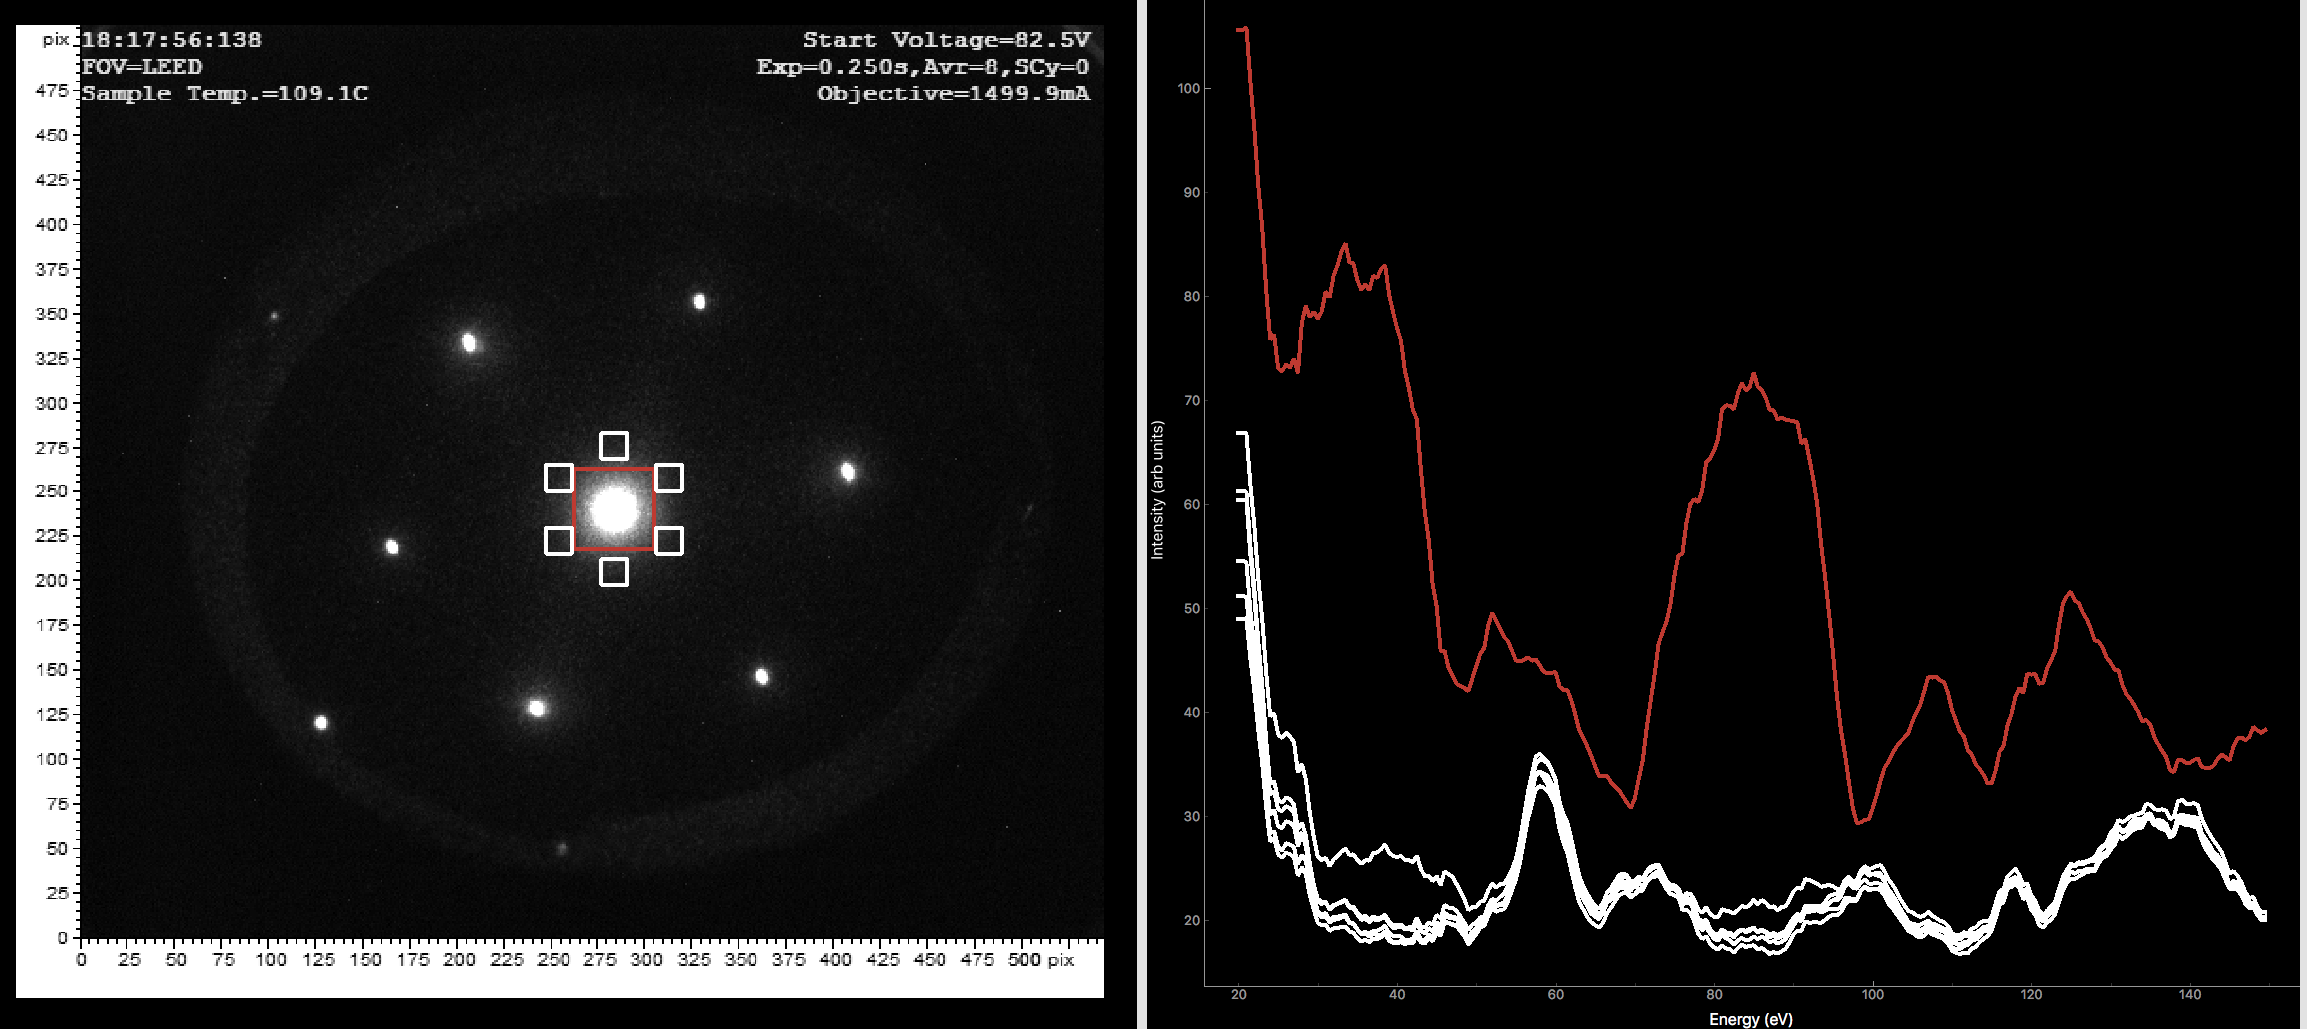
\includegraphics{BulkMoS2-LEED-IV-Background.png}
\caption{LEED-I(V) and Background from PLEASE}
\end{figure}

    \paragraph{Now we need to grab some information from the first file,
which contains the beam data for the (00) beam, the red curve in the
first figure. First we create two lists for Energy Values and Beam
Intensity Values. Then we parse the first text file for the required
data. The text files from PLEASE are output as tab-delimited files with
Energy in the first column and Intensity in the second column. So we can
simply read the lines of the text file, discard the first header line,
and split the lines bases on the TAB character to grab the relevant
information.}\label{now-we-need-to-grab-some-information-from-the-first-file-which-contains-the-beam-data-for-the-00-beam-the-red-curve-in-the-first-figure.-first-we-create-two-lists-for-energy-values-and-beam-intensity-values.-then-we-parse-the-first-text-file-for-the-required-data.-the-text-files-from-please-are-output-as-tab-delimited-files-with-energy-in-the-first-column-and-intensity-in-the-second-column.-so-we-can-simply-read-the-lines-of-the-text-file-discard-the-first-header-line-and-split-the-lines-bases-on-the-tab-character-to-grab-the-relevant-information.}

    \begin{Verbatim}[commandchars=\\\{\}]
{\color{incolor}In [{\color{incolor}4}]:} \PY{c+c1}{\PYZsh{} Get Energy values and (00) Beam Intensity Values}
        \PY{n}{Energy} \PY{o}{=} \PY{p}{[}\PY{p}{]}
        \PY{n}{Beam\PYZus{}Intensity} \PY{o}{=} \PY{p}{[}\PY{p}{]}
        \PY{k}{with} \PY{n+nb}{open}\PY{p}{(}\PY{n}{files}\PY{p}{[}\PY{l+m+mi}{0}\PY{p}{]}\PY{p}{,} \PY{l+s+s1}{\PYZsq{}}\PY{l+s+s1}{r}\PY{l+s+s1}{\PYZsq{}}\PY{p}{)} \PY{k}{as} \PY{n}{f}\PY{p}{:}
            \PY{n}{lines} \PY{o}{=} \PY{n}{f}\PY{o}{.}\PY{n}{readlines}\PY{p}{(}\PY{p}{)}\PY{p}{[}\PY{l+m+mi}{1}\PY{p}{:}\PY{p}{]}  \PY{c+c1}{\PYZsh{} discard header}
        \PY{k}{for} \PY{n}{line} \PY{o+ow}{in} \PY{n}{lines}\PY{p}{:}
            \PY{n}{Energy}\PY{o}{.}\PY{n}{append}\PY{p}{(}\PY{n+nb}{float}\PY{p}{(}\PY{n}{line}\PY{o}{.}\PY{n}{split}\PY{p}{(}\PY{l+s+s2}{\PYZdq{}}\PY{l+s+se}{\PYZbs{}t}\PY{l+s+s2}{\PYZdq{}}\PY{p}{)}\PY{p}{[}\PY{l+m+mi}{0}\PY{p}{]}\PY{p}{)}\PY{p}{)}
            \PY{n}{Beam\PYZus{}Intensity}\PY{o}{.}\PY{n}{append}\PY{p}{(}\PY{n+nb}{float}\PY{p}{(}\PY{n}{line}\PY{o}{.}\PY{n}{split}\PY{p}{(}\PY{l+s+s2}{\PYZdq{}}\PY{l+s+se}{\PYZbs{}t}\PY{l+s+s2}{\PYZdq{}}\PY{p}{)}\PY{p}{[}\PY{l+m+mi}{1}\PY{p}{]}\PY{p}{)}\PY{p}{)}
\end{Verbatim}


    \paragraph{To double check that we got the correct data, let's plot the
raw I(V) curve using the two lists we just
created}\label{to-double-check-that-we-got-the-correct-data-lets-plot-the-raw-iv-curve-using-the-two-lists-we-just-created}

    \begin{Verbatim}[commandchars=\\\{\}]
{\color{incolor}In [{\color{incolor}5}]:} \PY{n}{plt}\PY{o}{.}\PY{n}{figure}\PY{p}{(}\PY{n}{dpi}\PY{o}{=}\PY{l+m+mi}{120}\PY{p}{)}
        \PY{n}{plt}\PY{o}{.}\PY{n}{plot}\PY{p}{(}\PY{n}{Energy}\PY{p}{,} \PY{n}{Beam\PYZus{}Intensity}\PY{p}{)}
        \PY{n}{plt}\PY{o}{.}\PY{n}{xlabel}\PY{p}{(}\PY{l+s+s2}{\PYZdq{}}\PY{l+s+s2}{Energy [eV]}\PY{l+s+s2}{\PYZdq{}}\PY{p}{)}
        \PY{n}{plt}\PY{o}{.}\PY{n}{ylabel}\PY{p}{(}\PY{l+s+s2}{\PYZdq{}}\PY{l+s+s2}{Raw Beam Intensity [arb. units]}\PY{l+s+s2}{\PYZdq{}}\PY{p}{)}
        \PY{n}{plt}\PY{o}{.}\PY{n}{title}\PY{p}{(}\PY{l+s+s2}{\PYZdq{}}\PY{l+s+s2}{Uncorrected Beam data}\PY{l+s+s2}{\PYZdq{}}\PY{p}{)}
\end{Verbatim}


\begin{Verbatim}[commandchars=\\\{\}]
{\color{outcolor}Out[{\color{outcolor}5}]:} <matplotlib.text.Text at 0x11c59b860>
\end{Verbatim}

    \begin{center}
    \adjustimage{max size={0.9\linewidth}{0.9\paperheight}}{output_13_1.png}
    \end{center}
    { \hspace*{\fill} \\}

    \paragraph{Next we need to get the intensity of the background beams as
output by PLEASE, which are the white curves in the first figure. We are
going to sum the intensity for each energy step then average by the
number of beams at the end. We start by creating a list of zeros with
the same length as Beam\_Intensity. Then we add the intensity parsed
from the text files at each step through energy
space.}\label{next-we-need-to-get-the-intensity-of-the-background-beams-as-output-by-please-which-are-the-white-curves-in-the-first-figure.-we-are-going-to-sum-the-intensity-for-each-energy-step-then-average-by-the-number-of-beams-at-the-end.-we-start-by-creating-a-list-of-zeros-with-the-same-length-as-beam_intensity.-then-we-add-the-intensity-parsed-from-the-text-files-at-each-step-through-energy-space.}

    \begin{Verbatim}[commandchars=\\\{\}]
{\color{incolor}In [{\color{incolor}6}]:} \PY{n}{Background\PYZus{}Intensity} \PY{o}{=} \PY{p}{[}\PY{l+m+mi}{0}\PY{p}{]}\PY{o}{*}\PY{n+nb}{len}\PY{p}{(}\PY{n}{Beam\PYZus{}Intensity}\PY{p}{)}
\end{Verbatim}


    \begin{Verbatim}[commandchars=\\\{\}]
{\color{incolor}In [{\color{incolor}7}]:} \PY{k}{for} \PY{n}{fl} \PY{o+ow}{in} \PY{n}{files}\PY{p}{[}\PY{l+m+mi}{1}\PY{p}{:}\PY{p}{]}\PY{p}{:}  \PY{c+c1}{\PYZsh{} loop over all background files}
            \PY{k}{with} \PY{n+nb}{open}\PY{p}{(}\PY{n}{fl}\PY{p}{,} \PY{l+s+s1}{\PYZsq{}}\PY{l+s+s1}{r}\PY{l+s+s1}{\PYZsq{}}\PY{p}{)} \PY{k}{as} \PY{n}{f}\PY{p}{:}
                \PY{n}{lines} \PY{o}{=} \PY{n}{f}\PY{o}{.}\PY{n}{readlines}\PY{p}{(}\PY{p}{)}\PY{p}{[}\PY{l+m+mi}{1}\PY{p}{:}\PY{p}{]}  \PY{c+c1}{\PYZsh{} discard header}
            \PY{k}{for} \PY{n}{idx}\PY{p}{,} \PY{n}{line} \PY{o+ow}{in} \PY{n+nb}{enumerate}\PY{p}{(}\PY{n}{lines}\PY{p}{)}\PY{p}{:}
                \PY{c+c1}{\PYZsh{} Sum intensity for all background beams}
                \PY{n}{Background\PYZus{}Intensity}\PY{p}{[}\PY{n}{idx}\PY{p}{]} \PY{o}{+}\PY{o}{=} \PY{n+nb}{float}\PY{p}{(}\PY{n}{line}\PY{o}{.}\PY{n}{split}\PY{p}{(}\PY{l+s+s2}{\PYZdq{}}\PY{l+s+se}{\PYZbs{}t}\PY{l+s+s2}{\PYZdq{}}\PY{p}{)}\PY{p}{[}\PY{l+m+mi}{1}\PY{p}{]}\PY{p}{)}
\end{Verbatim}


    \paragraph{What have now is a list of the total background intensity
from all beams output by PLEASE. Next, we want to average the list by
the number of beams to get the average background
intensity.}\label{what-have-now-is-a-list-of-the-total-background-intensity-from-all-beams-output-by-please.-next-we-want-to-average-the-list-by-the-number-of-beams-to-get-the-average-background-intensity.}

    \begin{Verbatim}[commandchars=\\\{\}]
{\color{incolor}In [{\color{incolor}8}]:} \PY{c+c1}{\PYZsh{} Average the total intensity by the number of background beams (6)}
        \PY{n}{Background\PYZus{}Intensity} \PY{o}{=} \PY{p}{[}\PY{n}{i}\PY{o}{/}\PY{l+m+mi}{6} \PY{k}{for} \PY{n}{i} \PY{o+ow}{in} \PY{n}{Background\PYZus{}Intensity}\PY{p}{]}
\end{Verbatim}


    \paragraph{Again, let's double check that this is correct by plotting
the raw Beam Intensity and the Average Background
Intensity.}\label{again-lets-double-check-that-this-is-correct-by-plotting-the-raw-beam-intensity-and-the-average-background-intensity.}

    \begin{Verbatim}[commandchars=\\\{\}]
{\color{incolor}In [{\color{incolor}9}]:} \PY{n}{fig}\PY{p}{,} \PY{n}{ax} \PY{o}{=} \PY{n}{plt}\PY{o}{.}\PY{n}{subplots}\PY{p}{(}\PY{n}{nrows}\PY{o}{=}\PY{l+m+mi}{1}\PY{p}{,} \PY{n}{ncols}\PY{o}{=}\PY{l+m+mi}{1}\PY{p}{,} \PY{n}{dpi}\PY{o}{=}\PY{l+m+mi}{120}\PY{p}{)}
        \PY{n}{ax}\PY{o}{.}\PY{n}{plot}\PY{p}{(}\PY{n}{Energy}\PY{p}{,} \PY{n}{Beam\PYZus{}Intensity}\PY{p}{,} \PY{n}{label}\PY{o}{=}\PY{l+s+s2}{\PYZdq{}}\PY{l+s+s2}{Raw Beam Intensity}\PY{l+s+s2}{\PYZdq{}}\PY{p}{)}
        \PY{n}{ax}\PY{o}{.}\PY{n}{plot}\PY{p}{(}\PY{n}{Energy}\PY{p}{,} \PY{n}{Background\PYZus{}Intensity}\PY{p}{,} \PY{n}{label}\PY{o}{=}\PY{l+s+s2}{\PYZdq{}}\PY{l+s+s2}{Average Background Intensity}\PY{l+s+s2}{\PYZdq{}}\PY{p}{)}
        \PY{n}{ax}\PY{o}{.}\PY{n}{legend}\PY{p}{(}\PY{p}{)}
        \PY{n}{plt}\PY{o}{.}\PY{n}{xlabel}\PY{p}{(}\PY{l+s+s2}{\PYZdq{}}\PY{l+s+s2}{Energy [eV]}\PY{l+s+s2}{\PYZdq{}}\PY{p}{)}
        \PY{n}{plt}\PY{o}{.}\PY{n}{ylabel}\PY{p}{(}\PY{l+s+s2}{\PYZdq{}}\PY{l+s+s2}{Intensity [arb. units]}\PY{l+s+s2}{\PYZdq{}}\PY{p}{)}
        \PY{n}{plt}\PY{o}{.}\PY{n}{title}\PY{p}{(}\PY{l+s+s2}{\PYZdq{}}\PY{l+s+s2}{Comparing Uncorrected Beam I(V) to Average Background}\PY{l+s+s2}{\PYZdq{}}\PY{p}{)}
\end{Verbatim}


\begin{Verbatim}[commandchars=\\\{\}]
{\color{outcolor}Out[{\color{outcolor}9}]:} <matplotlib.text.Text at 0x11c8d9358>
\end{Verbatim}

    \begin{center}
    \adjustimage{max size={0.9\linewidth}{0.9\paperheight}}{output_20_1.png}
    \end{center}
    { \hspace*{\fill} \\}

    \paragraph{Finally, let's perform a simple background subtraction by
taking the Raw Beam Intensity and subtracting the Average Background
Intensity for each step through energy
space.}\label{finally-lets-perform-a-simple-background-subtraction-by-taking-the-raw-beam-intensity-and-subtracting-the-average-background-intensity-for-each-step-through-energy-space.}

    \begin{Verbatim}[commandchars=\\\{\}]
{\color{incolor}In [{\color{incolor}10}]:} \PY{c+c1}{\PYZsh{} Subtract Background from Beam}
         \PY{n}{Corrected\PYZus{}Beam\PYZus{}Intensity} \PY{o}{=} \PY{p}{[}\PY{n}{Beam\PYZus{}Intensity}\PY{p}{[}\PY{n}{idx}\PY{p}{]} \PY{o}{\PYZhy{}} \PY{n}{Background\PYZus{}Intensity}\PY{p}{[}\PY{n}{idx}\PY{p}{]}
                                         \PY{k}{for} \PY{n}{idx}\PY{p}{,} \PY{n}{\PYZus{}} \PY{o+ow}{in} \PY{n+nb}{enumerate}\PY{p}{(}\PY{n}{Beam\PYZus{}Intensity}\PY{p}{)}\PY{p}{]}
\end{Verbatim}


    \begin{Verbatim}[commandchars=\\\{\}]
{\color{incolor}In [{\color{incolor}11}]:} \PY{n}{fig}\PY{p}{,} \PY{n}{ax} \PY{o}{=} \PY{n}{plt}\PY{o}{.}\PY{n}{subplots}\PY{p}{(}\PY{n}{nrows}\PY{o}{=}\PY{l+m+mi}{1}\PY{p}{,} \PY{n}{ncols}\PY{o}{=}\PY{l+m+mi}{1}\PY{p}{,} \PY{n}{dpi}\PY{o}{=}\PY{l+m+mi}{120}\PY{p}{)}
         \PY{n}{ax}\PY{o}{.}\PY{n}{plot}\PY{p}{(}\PY{n}{Energy}\PY{p}{,} \PY{n}{Beam\PYZus{}Intensity}\PY{p}{,} \PY{n}{label}\PY{o}{=}\PY{l+s+s2}{\PYZdq{}}\PY{l+s+s2}{Raw Beam Intensity}\PY{l+s+s2}{\PYZdq{}}\PY{p}{)}
         \PY{n}{ax}\PY{o}{.}\PY{n}{plot}\PY{p}{(}\PY{n}{Energy}\PY{p}{,} \PY{n}{Background\PYZus{}Intensity}\PY{p}{,} \PY{n}{label}\PY{o}{=}\PY{l+s+s2}{\PYZdq{}}\PY{l+s+s2}{Average Background Intensity}\PY{l+s+s2}{\PYZdq{}}\PY{p}{)}
         \PY{n}{ax}\PY{o}{.}\PY{n}{plot}\PY{p}{(}\PY{n}{Energy}\PY{p}{,} \PY{n}{Corrected\PYZus{}Beam\PYZus{}Intensity}\PY{p}{,} \PY{n}{label}\PY{o}{=}\PY{l+s+s2}{\PYZdq{}}\PY{l+s+s2}{Corrected Beam Intensity}\PY{l+s+s2}{\PYZdq{}}\PY{p}{)}
         \PY{n}{ax}\PY{o}{.}\PY{n}{legend}\PY{p}{(}\PY{p}{)}
         \PY{n}{plt}\PY{o}{.}\PY{n}{xlabel}\PY{p}{(}\PY{l+s+s2}{\PYZdq{}}\PY{l+s+s2}{Energy [eV]}\PY{l+s+s2}{\PYZdq{}}\PY{p}{)}
         \PY{n}{plt}\PY{o}{.}\PY{n}{ylabel}\PY{p}{(}\PY{l+s+s2}{\PYZdq{}}\PY{l+s+s2}{Intensity [arb. units]}\PY{l+s+s2}{\PYZdq{}}\PY{p}{)}
         \PY{n}{plt}\PY{o}{.}\PY{n}{title}\PY{p}{(}\PY{l+s+s2}{\PYZdq{}}\PY{l+s+s2}{Comparing Raw Beam Data to Corrected Data}\PY{l+s+s2}{\PYZdq{}}\PY{p}{)}
\end{Verbatim}


\begin{Verbatim}[commandchars=\\\{\}]
{\color{outcolor}Out[{\color{outcolor}11}]:} <matplotlib.text.Text at 0x11ca99b38>
\end{Verbatim}

    \begin{center}
    \adjustimage{max size={0.9\linewidth}{0.9\paperheight}}{output_23_1.png}
    \end{center}
    { \hspace*{\fill} \\}

    \subsection{Here's the final result}\label{heres-the-final-result}

    \begin{Verbatim}[commandchars=\\\{\}]
{\color{incolor}In [{\color{incolor}12}]:} \PY{n}{plt}\PY{o}{.}\PY{n}{figure}\PY{p}{(}\PY{n}{dpi}\PY{o}{=}\PY{l+m+mi}{120}\PY{p}{)}
         \PY{n}{plt}\PY{o}{.}\PY{n}{plot}\PY{p}{(}\PY{n}{Energy}\PY{p}{,} \PY{n}{Corrected\PYZus{}Beam\PYZus{}Intensity}\PY{p}{)}
         \PY{n}{plt}\PY{o}{.}\PY{n}{xlabel}\PY{p}{(}\PY{l+s+s2}{\PYZdq{}}\PY{l+s+s2}{Energy [eV]}\PY{l+s+s2}{\PYZdq{}}\PY{p}{)}
         \PY{n}{plt}\PY{o}{.}\PY{n}{ylabel}\PY{p}{(}\PY{l+s+s2}{\PYZdq{}}\PY{l+s+s2}{Corrected Intensity [arb. units]}\PY{l+s+s2}{\PYZdq{}}\PY{p}{)}
         \PY{n}{plt}\PY{o}{.}\PY{n}{title}\PY{p}{(}\PY{l+s+s2}{\PYZdq{}}\PY{l+s+s2}{Background Corrected I(V) from Bulk MoS2 (00) Beam}\PY{l+s+s2}{\PYZdq{}}\PY{p}{)}
\end{Verbatim}


\begin{Verbatim}[commandchars=\\\{\}]
{\color{outcolor}Out[{\color{outcolor}12}]:} <matplotlib.text.Text at 0x11cb221d0>
\end{Verbatim}

    \begin{center}
    \adjustimage{max size={0.9\linewidth}{0.9\paperheight}}{output_25_1.png}
    \end{center}
    { \hspace*{\fill} \\}

    \subsection{Bonus: The electron beam we are analyzing is the (00) beam,
which is the spectrally reflected beam. Thus we can rescale the Y-axis
and plot Electron Reflectivity vs
Energy}\label{bonus-the-electron-beam-we-are-analyzing-is-the-00-beam-which-is-the-spectrally-reflected-beam.-thus-we-can-rescale-the-y-axis-and-plot-electron-reflectivity-vs-energy}

    \begin{Verbatim}[commandchars=\\\{\}]
{\color{incolor}In [{\color{incolor}13}]:} \PY{n}{max\PYZus{}int} \PY{o}{=} \PY{n+nb}{max}\PY{p}{(}\PY{n}{Corrected\PYZus{}Beam\PYZus{}Intensity}\PY{p}{)}
         \PY{n}{plt}\PY{o}{.}\PY{n}{figure}\PY{p}{(}\PY{n}{dpi}\PY{o}{=}\PY{l+m+mi}{120}\PY{p}{)}
         \PY{n}{plt}\PY{o}{.}\PY{n}{plot}\PY{p}{(}\PY{n}{Energy}\PY{p}{,} \PY{p}{[}\PY{n}{k}\PY{o}{/}\PY{n}{max\PYZus{}int} \PY{k}{for} \PY{n}{k} \PY{o+ow}{in} \PY{n}{Corrected\PYZus{}Beam\PYZus{}Intensity}\PY{p}{]}\PY{p}{)}  \PY{c+c1}{\PYZsh{}}
         \PY{n}{plt}\PY{o}{.}\PY{n}{xlabel}\PY{p}{(}\PY{l+s+s2}{\PYZdq{}}\PY{l+s+s2}{Energy [eV]}\PY{l+s+s2}{\PYZdq{}}\PY{p}{)}
         \PY{n}{plt}\PY{o}{.}\PY{n}{ylabel}\PY{p}{(}\PY{l+s+s2}{\PYZdq{}}\PY{l+s+s2}{Corrected Electron Reflectivity}\PY{l+s+s2}{\PYZdq{}}\PY{p}{)}
         \PY{n}{plt}\PY{o}{.}\PY{n}{title}\PY{p}{(}\PY{l+s+s2}{\PYZdq{}}\PY{l+s+s2}{Background Corrected Electron Reflectivity from Bulk MoS2 (00) Beam}\PY{l+s+s2}{\PYZdq{}}\PY{p}{)}
\end{Verbatim}


\begin{Verbatim}[commandchars=\\\{\}]
{\color{outcolor}Out[{\color{outcolor}13}]:} <matplotlib.text.Text at 0x11ccb98d0>
\end{Verbatim}

    \begin{center}
    \adjustimage{max size={0.9\linewidth}{0.9\paperheight}}{output_27_1.png}
    \end{center}
    { \hspace*{\fill} \\}


    % Add a bibliography block to the postdoc



    \end{document}
